\title{Changes on CRAN}
\subtitle{2022-07-01 to 2022-10-31}
\author{by Kurt Hornik, Uwe Ligges and Achim Zeileis}
\maketitle

\sloppy

\inputencoding{utf8}

In the past 4 months, 664 new packages were added to the CRAN package
repository.  154~packages were unarchived, 353 were archived and 6 had
to be removed.  The following shows the growth of the number of active
packages in the CRAN package repository:

\begin{figure}[h]
  \centering
  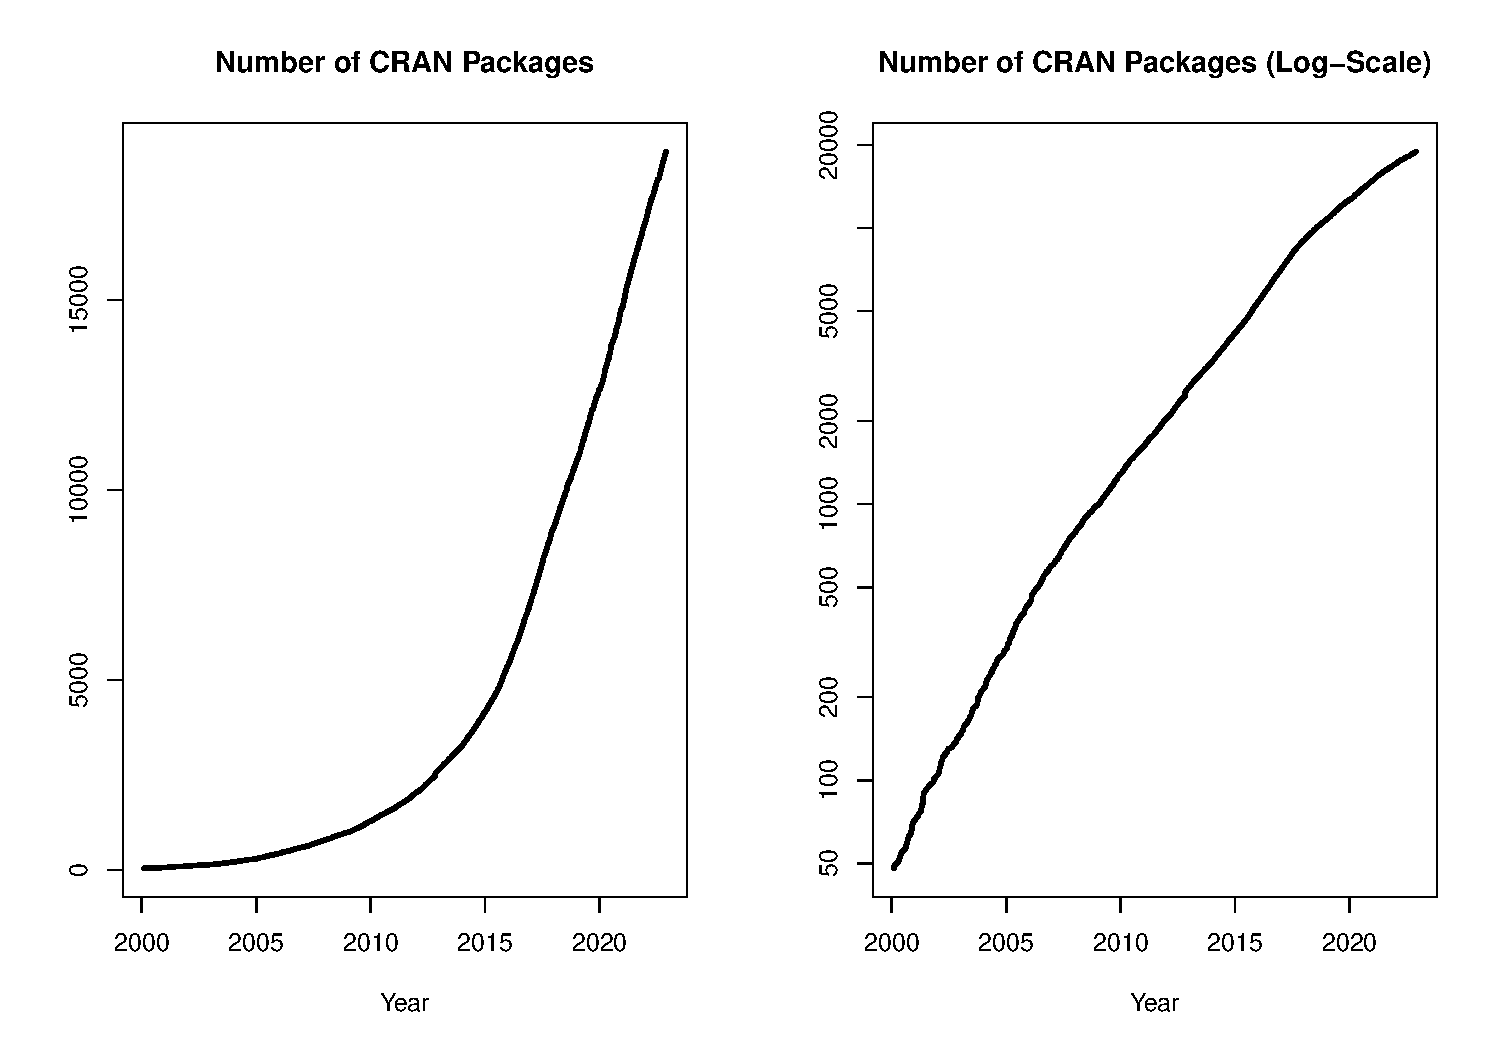
\includegraphics[width=5in]{cran_growth}
\end{figure}

\noindent
On 2022-10-31, the number of active packages was around 18730.

% \subsection{Changes in the CRAN Repository Policy}

%% cd ~/src/org/R-project/R-dev-web/CRAN/Policy
%% svn diff -r{2022-09-01}:{2022-10-31}

\subsection{CRAN package submissions}

 From September 2022 to October 2022 CRAN received 5227 package submissions.
For these, 9429~actions took place of which 6070 (64\%) were auto 
processed actions and 3359 (36\%) manual actions.

Minus some special cases, a summary of the auto-processed and manually 
triggered actions follows:
\begin{center}
\setlength{\tabcolsep}{2pt}
\begin{tabular}{l|rrrrrrrr}
  & archive & inspect & newbies & pending & pretest & publish & recheck 
& waiting \\ \hline
auto & 1335 & 1211 & 926 & 0 & 0 & 1560 & 513 & 525 \\
manual & 1250 & 35 & 325 & 232 & 39 & 1054 & 353 & 71
\end{tabular}
\end{center}

These include the final decisions for the submissions which were
\begin{center}
\begin{tabular}{l|rr}
  & archive & publish \\ \hline
auto & 1283 (25.1\%) & 1239 (24.3\%) \\
manual & 1222 (23.9\%) & 1361 (26.7\%)
\end{tabular}
\end{center}
where we only count those as \emph{auto} processed whose publication or
rejection happened automatically in all steps.

\subsection{CRAN mirror security}

%% ~/Work/R/CRAN_Admin/cran_secure_http_and_rsync.R

Currently, there are 100 official CRAN mirrors, 81 of which provide both
secure downloads via \samp{https} \emph{and} use secure mirroring from
the CRAN master (via rsync through ssh tunnels).  Since the~R 3.4.0
release, \code{chooseCRANmirror()} offers these mirrors in preference to
the others which are not fully secured (yet).

\subsection{CRAN Task View Initiative}

There are three new task views:
\begin{description}
 \item[\href{https://CRAN.R-project.org/view=Agriculture}{Agricultural Science}]
  Maintained by Julia Piaskowski, Adam Sparks, and Janet Williams.
 \item[\href{https://CRAN.R-project.org/view=MixedModels}{Mixed, Multilevel, and Hierarchical Models in R}]
  Maintained by Ben Bolker, Julia Piaskowski, Emi Tanaka, Phillip Alday,
  and Wolfgang Viechtbauer.
 \item[\href{https://CRAN.R-project.org/view=Phylogenetics}{Phylogenetics}]
  Maintained by William Gearty, Brian O'Meara, Jacob Berv, Gustavo
  A. Ballen, Diniz Ferreira, Hilmar Lapp, Lars Schmitz, Martin R. Smith,
  Nathan S. Upham, and Jonathan A. Nations. 
\end{description}

Currently there are 42 task views (see
\url{https://cran.r-project.org/web/views/}), with median and mean
numbers of CRAN packages covered 102 and 115, respectively.  Overall,
these task views cover 4015~CRAN packages, which is about 21\% of all
active CRAN packages.

\address{Kurt Hornik \\
  WU Wirtschaftsuniversit\"at Wien, Austria \\
  \email{Kurt.Hornik@R-project.org}}

\address{Uwe Ligges \\
  TU Dortmund, Germany \\
  \email{Uwe.Ligges@R-project.org}}

\address{Achim Zeileis \\
  Universit\"at Innsbruck, Austria \\
  \email{Achim.Zeileis@R-project.org}}

